\chapter{Pré-Processamento dos Verbos para Redes Neurais}
\label{ch:02}

Este capítulo tratará de uma das partes mais importantes da modelagem em redes neurais: o pré-processamento dos dados. Muito se discute sobre o desenvolvimento de novas técnicas e arquiteturas, mas nem sempre a mesma importância é dada para esse estágio da modelagem - que é, na maioria das vezes, onde se dedica mais tempo. 

Neste trabalho, os dados de interesse são \textit{verbos}, e para um computador, um verbo é apenas uma sequência de caracteres. Ademais, um modelo de Redes Neurais é um modelo computacional, e para que o modelo funcione, é necessário preparar os dados para que eles estejam em um formato adequado para os cálculos que serão realizados. Desse modo, mesmo sem adentrar na parte teórica do funcionamento do modelo, já cabe discutir de que forma os verbos serão inseridos. Em suma, os modelos de redes neurais são alimentados com \textit{vetores numéricos} (ou \textit{arrays}). Esses vetores são essencialmente uma lista de números (por ex. [0, 1, 2, 3]). Assim, pré-processar os verbos para a alimentação do modelo significa encontrar uma \textit{representação vetorial} para cada um deles. Ainda, teremos que todos os verbos serão representados por vetores de comprimentos iguais, e que será este mesmo comprimento que definirá a dimensão (número de nódulos) da primeira camada da rede (a camada de \textit{input}). Além disso, também é neste momento em que definiremos o recorte dos dados - o nível de abstração do estudo, por assim dizer. Em outras palavras, isso significa que podemos recortar um verbo de diversas maneiras: podemos considerar que verbos são uma sequência de letras, ou uma sequência de fones, uma sequência de morfemas, etc. Porém, ao fazermos este recorte, estaremos automaticamente enviesando o resultado final do estudo. Por exemplo, se optarmos por representar um verbo utilizando a escrita ortográfica do mesmo, o modelo falhará em encontrar as relações mais sutis entre os elementos fonéticos desse verbo.

Desse modo, fica evidente a importância desta etapa. Falaremos primeiramente sobre o pré-processamento utilizado por \cite{rumelhart:1986}. Em seguida, será exibido o pré-processamento utilizado neste trabalho para a alimentação do \textit{Encoder-Decoder} desenvolvido. Ainda, em questão de terminologia, por vezes o termo \textit{codificação} será utilizado como opção a pré-processamento.  

\section{Pré-Processamento de Rumelhart \& McClelland}
\label{sec:transcr}
A arquitetura do modelo utilizado por \cite{rumelhart:1986} era bastante limitada para o problema em questão. A limitação resultava do fato de que tanto os \textit{inputs} quantos os \textit{alvos} do modelo possuíam tamanhos variáveis. O \textit{input}, por exemplo, poderia ser “\textit{like}” ou “\textit{overtake}”, e os \textit{alvos}, “\textit{liked}” e “\textit{overtook}”. Entretanto, a arquitetura \textit{Feedforward} (Fig. \ref{fig:ffd}) é composta por um número fixo de nódulos em cada camada. Poderíamos supor simplesmente que cada nódulo representasse cada fone do alfabeto fonético. Dessa forma, o \textit{input} hipotético seria o conjunto de fones do verbo. Entretanto, ao fazermos isto, a rede perderia completamente a noção de sequência dos fones. Dada a limitação, Rumelhart e McClelland acabaram desenvolvendo um sistema de codificação composto por várias etapas. Utilizaremos o verbo “\textit{came}” como exemplo para detalhar cada um dos estágios de codificação utilizados pelos pesquisadores.

A primeira etapa consistiu na transcrição dos verbos utilizando um alfabeto compatível com o código ASCII (\cite{mackenzie1980coded}). O código ASCII é um código 
usado para representar textos em computadores. Ele codifica letras do alfabeto latino, sinais de pontuação e sinais matemáticos. A opção pela utilização do código ASCII é necessária, pois o código fonético não é interpretável pelas linguagens de programação. Segundo a chave de transcrição dos pesquisadores (Apêndice), o verbo “\textit{came}” foi transcrito para “\#\textit{kAm}\#”. O símbolo “\#” é utilizado para demarcar o início e o final do verbo. 

Em seguida, as transcrições foram reestruturadas em \textit{trigramas}. Fazer isso significa analisar a sequência do verbo de três em três segmentos, ou seja, nessa etapa, a sequência “\#\textit{kAm}\#” passou a ser tratada como “\#\textit{kA}” + “\textit{kAm}” + “\textit{Am}\#”. Cada um desses trigramas é chamado de \textit{Wickelphone}, estrutura nomeada por \cite{wickelgren:1969}.

Na sequência, os autores apresentam uma nova estrutura intitulada de \textit{Wickelfeatures}. Os \textit{Wickelfeatures} são justamente as tríades de traços fonéticos introduzidas no Cap. \ref{ch:01}. Como visto na Tabela \ref{tab:trigrams}, cada um dos fones pode ser descrito por algumas características relacionadas à execução dos seus respectivos sons. Entretanto, as características dos trigramas formados podem ser combinadas de muitas formas, mais precisamente, $4^{3}$ possibilidades, visto que cada fone pode ser descrito por 4 traços (Apêndice (ref)). 

Assim, para a construção dos nódulos do modelo, \cite{rumelhart:1986} computaram todos os \textit{Wickelfeatures} possíveis entre os verbos e excluíram alguns redundantes para simplificar a computação. Ao final, os \textit{Wickelfeatures} dos verbos foram mapeados como chaves em um dicionário de tamanho fixo (um vetor) em que os valores poderiam assumir somente 0 ou 1; 1 caso aquele \textit{Wickelfeature} estivesse presente no verbo e 0 caso contrário. A Figura \ref{fig:wick} ilustra o esquema de codificação para o verbo “came”. 

\definecolor{blue}{RGB}{159, 192, 176}
\definecolor{green}{RGB}{160, 227, 127}
\definecolor{orange}{RGB}{243, 188, 125}
\definecolor{red}{RGB}{253, 123, 84}
\definecolor{nephritis}{RGB}{39, 174, 96}
\definecolor{emerald}{RGB}{46, 204, 113}
\definecolor{turquoise}{RGB}{39, 174, 96}
\definecolor{green-sea}{RGB}{22, 160, 133}
\definecolor{purple}{RGB}{181, 124, 215}
% Tikzstyles for Computation Graphs

% nodes
\tikzstyle{noop} = [circle, draw=none, fill=red, minimum size = 10pt]
\tikzstyle{op} = [circle, draw=red, line width=1.5pt, fill=red!70, text=black, text centered, font=\bf \normalsize, minimum size = 25pt]

\tikzstyle{opintense} = [circle, draw=red, line width=1.5pt, fill=red!150, text=black, text centered, font=\bf \normalsize, minimum size = 25pt]


%new style
\tikzstyle{gp} = [circle, draw=red, line width=4pt, text=black, text centered, font=\bf \normalsize, minimum size = 4.cm]

\tikzstyle{box} = [rectangle, draw=red, line width=1.5pt, fill=red!70, text=black, align=center, font=\bf \normalsize, minimum size = 45pt]

\tikzstyle{box2} = [rectangle, draw=black, line width=0.9pt, text=black, align=center, font=\bf \normalsize, minimum size = 20pt]

\tikzstyle{box3} = [rectangle, draw=black, line width=0.9pt, fill=black, text=black, align=center, font=\bf \normalsize, minimum size = 20pt]

\tikzstyle{state} = [circle, draw=blue, line width=1.5pt, fill=blue!70, text=black, text centered, font=\bf \normalsize, minimum size = 25pt]

\tikzstyle{output} = [circle, draw=purple, line width=1.5pt, fill=purple!70, text=black, text centered, font=\bf \normalsize, minimum size = 25pt]


\tikzstyle{gradient} = [circle, draw=nephritis, line width=1.5pt, fill=nephritis!60, text=black, text centered, font=\bf \normalsize, minimum size = 25pt]
\tikzstyle{textonly} = [draw=none, fill=none, text centered, font=\bf \normalsize]
\tikzstyle{boxtextonly} = [draw=none, fill=none, align=center, font=\bf \normalsize]

\tikzstyle{normal} = [circle, draw=black, line width=1.0pt, fill=none, text=black, text centered, font=\bf \normalsize, minimum size = 20pt]


% edges
\tikzstyle{tedge}  = [draw, thick, >=latex, ->]
\tikzstyle{tedge_dashed}  = [draw, thick, >=latex, ->, dashed]
\tikzstyle{nedge}  = [draw, thick, >=latex]
\tikzstyle{nedge_dashed}  = [draw, thick, >=latex, dashed]


% namedscope
\tikzstyle{namedscope} = [circle, draw=orange, line width=1.5pt, fill=orange!60, align=center, inner sep=0pt]
\begin{figure}[ht!]
\centering

\scalebox{1.0}{
\begin{tikzpicture}[H]

%vetor
\node[box2] (box1) {};
\node[box2, below=0pt of box1] (box2) {};
\node[box3, below=0pt of box2] (box3) {};
\node[box3, below=0pt of box3] (box4) {};
\node[textonly, below=0pt of box4] (box5) {\reflectbox{$\vdots$}};
\node[box3, below=0pt of box5] (box6) {};
\node[box3, below=0pt of box6] (box7) {};
\node[box2, below=0pt of box7] (box8) {};
\node[box3, below=0pt of box8] (box9) {};
\node[box2, below=0pt of box9] (box10) {};
\node[textonly, below=0pt of box10] (dim) {460x1};
\node[textonly, below=0pt of dim] (space) {};
%wickelfeatures
\node[textonly, right=20pt of box1] (wi1) {\#, oclusiva, média};
\node[textonly, right=20pt of box2] (wi2) {\#, anterior, fricativa};
\node[textonly, right=20pt of box3] (wi3) {\#, fricativa, vogal};
\node[textonly, right=20pt of box4] (wi4) {\#, contínua, anterior};
\node[textonly, right=20pt of box5] (wi5) {\reflectbox{$\vdots$}};
\node[textonly, right=20pt of box6] (wi6) {\#, não vozeada, aberta};
\node[textonly, right=20pt of box7] (wi7) {\#, contínua, posterior};
\node[textonly, right=20pt of box8] (wi8) {contínua, vogal, vogal };
\node[textonly, right=20pt of box9] (wi9) {contínua, vogal, líquida};
\node[textonly, right=20pt of box10] (wi10) {fricativa, posterior, \#};

%pré processamento
\node[textonly, left=230pt of box4] (verb1) {falar};
\node[textonly, below=10pt of verb1] (verb2) {fala};
\node[textonly, below=10pt of verb2] (verb3) {\#fala\#};

%trigramas
\node[textonly, right=20pt of verb1] (tri1) {\#,f,a};
\node[textonly, below=10pt of tri1] (tri2) {f,a,l};
\node[textonly, below=10pt of tri2] (tri3) {a,l,a};
\node[textonly, below=10pt of tri3] (tri4) {l,a,\#};

%features
\node[textonly, left=50pt of box2] (f1) {\#,cont,vogal};
\node[textonly, below=0pt of f1] (f2) {\#,cont,aberta};
\node[textonly, below=0pt of f2] (f3) {\#,cont,anterior};
\node[textonly, below=0pt of f3] (f4) {\#,cont,baixa};
\node[textonly, below=0pt of f4] (f5) {\reflectbox{$\vdots$}};
\end{tikzpicture}
}\caption{Esquema de Codificação de Wickelfeatures} 
\label{fig:wick}
\end{figure}

Como comentado no Cap. \ref{ch:01}, o modelo de \cite{rumelhart:1986} conseguiu alto desempenho nos dados de treinamento. Entretanto, a arquitetura do tipo \textit{Feedforward} não é a mais adequada para esse tipo de problema. Em primeiro lugar, o esquema de codificação proposto é bastante limitado, visto que os vetores de \textit{input} da rede conseguem marcar apenas a presença ou ausência dos \textit{Wickelfeatures}. Como um exemplo do problema, podemos analisar o verbo  \textit{understand}. A Tabela \ref{tab:wickeldertan} exibe uma comparação entre os \textit{Wickelfeatures} dos trigramas \textit{der} e \textit{tan}, ambos presentes no verbo de exemplo.

\begin{table}[!htb]
    \begin{minipage}{.5\linewidth}
      \centering
      \caption{}
        \begin{tabular}{ccc}
        d                    & e                    & r                    \\ \hline
        consoante            & vogal                & consoante            \\
        sonora               & frontal              & líquida              \\
        stop                 & short                & média                \\
        média               & low                  & sonora               \\
        \multicolumn{1}{l}{} & \multicolumn{1}{l}{} & \multicolumn{1}{l}{} \\
        \multicolumn{1}{l}{} & \multicolumn{1}{l}{} & \multicolumn{1}{l}{} \\
        \multicolumn{1}{l}{} & \multicolumn{1}{l}{} & \multicolumn{1}{l}{}
        \end{tabular}
        %\caption{Wickelfeatures do Trigrama der}
        \label{tab:der}
    \end{minipage}%
    \begin{minipage}{.5\linewidth}
      \centering
        \caption{}

    \begin{tabular}{ccc}
    t                    & a                    & n                    \\ \hline
    consoante            & vogal                & consoante            \\
    surda                & frontal              & líquida              \\
    stop                 & short                & média                \\
    média                & low                  & sonora               \\
    \multicolumn{1}{l}{} & \multicolumn{1}{l}{} & \multicolumn{1}{l}{} \\
    \multicolumn{1}{l}{} & \multicolumn{1}{l}{} & \multicolumn{1}{l}{} \\
    \multicolumn{1}{l}{} & \multicolumn{1}{l}{} & \multicolumn{1}{l}{}
    \end{tabular}
    %\caption{Wickelfeatures do Trigrama tan}
    \label{tab:tan}
    \end{minipage} 
\caption{\textit{Wickelfeatures} de \textit{der} e \textit{tan}}
\label{tab:wickeldertan}
\end{table}


Observa-se na Tabela \ref{tab:wickeldertan} que muitos \textit{Wickelfeatures} coincidem apesar dos dois trigramas serem completamente diferentes. 

Assim como os verbos tem que ser processados para entrarem nos modelos como vetores, a saída do modelo também precisa ser decodificada para reconstruir um verbo -  esse é o esquema de \textit{decodificação} dos \textit{outputs} do modelo. A decodificação envolvia um esquema também composto por várias etapas. De maneira simplificada, \cite{rumelhart:1986} elencaram os trigramas (\textit{Wickelphones}) candidatos para cada verbo e estes “competiam” pelos vetores de \textit{Wickelfeatures} mais relevantes da saída do modelo. Neste sentido, \cite{Pinker:1999} critica o modelo dos pesquisadores utilizando como exemplo a palavra “\textit{algalgal}” (uma palavra da língua Oykangand), cuja a repetição de \textit{Wickelfeatures} ocorre diversas vezes. Como a saída da rede FFD é também um vetor que guarda apenas a presença ou ausência dos traços, e não quantas vezes eles aparecem, o processo de decodificação apresenta problemas e a rede dificilmente acerta em casos de verbos maiores ou com repetições de \textit{Wickelfeatures}. As complicações observadas tanto na construção da codificação quanto na decodificação dos dados refletem a necessidade de uma arquitetura mais adequada para o problema em questão.

\section{Pré-Processamento para o Encoder-Decoder}

No caso da arquitetura \textit{Encoder-Decoder}, não há motivo para preocupação com relação à sequência dos dados, nem durante o processo de inserção, nem no processo de predição do modelo. A razão para tal ficará mais clara após os capítulos \ref{ch:03} e \ref{ch:05}. Entretanto, o que já pode ser adiantado é que não há a necessidade do tratamento dos verbos em trigramas, tão-pouco em \textit{Wickelfeatures}. Neste tipo de arquitetura, os verbos podem ser normalmente tratados como uma sequência de fones. Entretanto, mesmo com essa simplificação, existem múltiplas maneiras de se abordar essa questão. Este trabalho tem como objetivo estudar as relações entre os verbos em um nível fonético, portanto é importante que as representações vetoriais construídas levem isto em consideração.

Começaremos pela apresentação do Alfabeto Fonético Internacional (AFI), apresentado nas Tabelas \ref{tab:ipa1} e \ref{tab:ipa2}. O AFI é um sistema de notação fonética, criado pela Associação Fonética Internacional para promover uma padronização na transcrição de dados de diferentes idiomas. Ele organiza símbolos que representam unidades sonoras presentes nas línguas humanas a partir de características de execução dessas unidades. 

A Tabela \ref{tab:ipa1} reúne o conjunto dos sons consoantes e exibe na dimensão das colunas o ponto de articulação dos sons, isto é, o ponto de contato onde ocorre uma obstrução no trato vocal. A coluna “Bilabial”, por exemplo, corresponde à obstrução que ocorre nos lábios durante a produção dos seus respectivos fones. As linhas compõem os diferentes \textit{modos} de articulação possíveis, ou seja, as formas de obstrução da passagem de ar. A obstrução pode ser total como em \textbf{[p]} ou parcial como em \textbf{[s]}. Por fim, dentro de uma mesma célula pode ocorrer um som com ou sem a vibração das cordas vocais, é o caso do par \textbf{[p b]}. O símbolo da esquerda representa o som surdo e o símbolo da direita, sonoro. 

As vogais estão organizadas na Fig. \ref{fig:vowels_ipa}. As colunas dessa tabela se referem ao local de reprodução dos sons (com avanço ou recuo da língua), e as linhas, à altura da língua em relação ao céu da boca durante a execução do som. Quando os símbolos aparecem em pares, aquele da direita representa uma vogal arredondada (\cite{paraconhecer:2015}). Como um exemplo do funcionamento desta tabela, é interessante observar a execução da vogal \textbf{[u]} compará-la com a vogal \textbf{[o]}. Ao pronunciar ambas para uma comparação, nota-se o arredondamento dos lábios em ambas, porém a altura da língua durante a execução da segunda é levemente mais baixa que a altura da primeira. Para entender a questão de anterioridade/posterioridade, é interessante observar a movimentação (avanço e recuo) da língua durante a execução de \textbf{[e]} e \textbf{[o]}.

\begin{center}
\scalebox{0.8}{
    \begin{tabular}{|l|cc|cc|cc|cc|cc|cc|cc|cc|cc|cc|cc|}
%\begin{tabular}{|l|cc|}
        \hline & 
            \multicolumn{2}{|c|}{\footnotesize{Bilabial}} &					% Bilabial
            \multicolumn{2}{|c|}{\footnotesize{Labiodental}} & 			% Labiodental
            \multicolumn{2}{|c|}{\footnotesize{Dental}} & 					% Dental
            \multicolumn{2}{|c|}{\footnotesize{Alveolar}} & 				% Alveolar
            \multicolumn{2}{|c|}{\footnotesize{P-alveo.}} & 		% Post-alveolar
            \multicolumn{2}{|c|}{\footnotesize{Retroflexa}} & 				% Retroflex
            \multicolumn{2}{|c|}{\footnotesize{Palatal}} & 					% Palatal
            \multicolumn{2}{|c|}{\footnotesize{Velar}} & 					% Velar
            \multicolumn{2}{|c|}{\footnotesize{Uvular}} & 					% Uvular
            \multicolumn{2}{|c|}{\footnotesize{Faringal}} & 			% Pharyngeal
            \multicolumn{2}{|c|}{\footnotesize{Glotal}}  \\% Glottal

        \hline 
        Oclusiva &	% Plosive
            \circled{p} & \circled{b} &													% Bilabial
            &&														% Labiodental
            \multicolumn{3}{|r}{\circled{t}}&							% Dental
            \multicolumn{3}{l|}{\circled{d}}&							% Alveolar
                                                                        % Post-alveolar
            \ipa{\:t} & \ipa{\:d}&									% Retroflex
            c & \textbardotlessj &														% Palatal
            \circled{k} & \circled{g} &													% Velar
            q & \ipa{\;G} &										% Uvular
            & \BlankCell        &								% Pharyngeal
            \ipa{P}& \BlankCell         \\								% Glottal

        \hline Nasal & 							% Nasal
            & \circled{m} &													% Bilabial
            & \ipa{M} &											% Labiodental
            \multicolumn{3}{|r}{}&								% Dental
            \multicolumn{3}{l|}{\circled{n}}&							% Alveolar
                                                                        % Post-alveolar
            & \ipa{\:n} &														% Retroflex
            & \textltailn &														% Palatal
            & \circled{\ipa{N}} &														% Velar
            & N &														% Uvular
            \BlankCell        & \BlankCell        &		% Pharyngeal
            \BlankCell        & \BlankCell         \\		% Glottal

        \hline Vibrante &  								% Trill
            & \ipa{\;B}&											% Bilabial
            & &														% Labiodental
            \multicolumn{3}{|r}{}&								% Dental
            \multicolumn{3}{l|}{\circled{r}}&								% Alveolar
                                                                        % Post-alveolar
            & &														% Retroflex
            & &														% Palatal
            \BlankCell        & \BlankCell        &		% Velar
            & \ipa{\;R}&											% Uvular
            & &														% Pharyngeal
            \BlankCell        & \BlankCell         \\		% Glottal

        \hline Tepe &  						% Tap /Flap
            & &													% Bilabial
            & &														% Labiodental
            \multicolumn{3}{|r}{} &					% Dental
            \multicolumn{3}{l|}{\ipa{R}} &					% Alveolar
                                                                        % Post-alveolar
            & \ipa{\:r} &														% Retroflex
            & &														% Palatal
            \BlankCell        & \BlankCell        &		% Velar
            & &														% Uvular
            & &														% Pharyngeal
            \BlankCell        & \BlankCell         \\		% Glottal

        \hline Fricativa & 						% Fricative
            \ipa{F} & \ipa{B} &									% Bilabial
            \circled{f} & \circled{v} &													% Labiodental
            \ipa{T} & \ipa{D} &									% Dental
            \circled{s} & \circled{z} &													% Alveolar
            \circled{\ipa{S}} & \circled{\ipa{Z}} &									% Post-alveolar
            \ipa{\:s} & \ipa{\:z} &								% Retroflex
            \ipa{\c{c}} & \ipa{J} &								% Palatal
            \circled{x} & \ipa{G} &											% Velar
            \ipa{X} & \ipa{K} &									% Uvular
            \textcrh & \ipa{Q} &								% Pharyngeal
            h & \texthth \\										% Glottal

        \hline Fric. Lateral & 					% Lat. Fricative
            \BlankCell        & \BlankCell        &		% Bilabial
            \BlankCell        & \BlankCell        &		% Labiodental
            \multicolumn{3}{|r}{\textbeltl} &				% Dental
            \multicolumn{3}{l|}{\textlyoghlig} &			% Alveolar
                                                                        % Post-alveolar
            & &														% Retroflex
            & &														% Palatal
            & &														% Velar
            & &														% Uvular
            \BlankCell        & \BlankCell        			% Pharyngeal
            & \BlankCell        & \BlankCell         \\   % Glottal

        \hline Aprox. & 							% Approx.
            & &														% Bilabial
            & \ipa{V} &											% Labiodental
            \multicolumn{3}{|r}{}&								% Dental
            \multicolumn{3}{l|}{\ipa{\*r}} &					% Alveolar
                                                                        % Post-alveolar
            & \ipa{\:R} &											% Retroflex
            & j &														% Palatal
            & \textturnmrleg &									% Velar
            & &														% Uvular
            & &														% Pharyngeal
            \BlankCell        & \BlankCell         \\		% Glottal

        \hline Aprox. Lateral & 					% Lat. Approx
            \BlankCell        & \BlankCell        &		% Bilabial
            \BlankCell        & \BlankCell        &		% Labiodental
            \multicolumn{3}{|r}{}&								% Dental
            \multicolumn{3}{l|}{\circled{l}}&								% Alveolar
                                                                        % Post-alveolar
            & \textipa{\:l} &											% Retroflex
            & \textipa{L} &												% Palatal
            & \circled{\textipa{\;L}} &											% Velar
            & &														% Uvular
            \BlankCell        & \BlankCell        &		% Pharyngeal
            \BlankCell        & \BlankCell         \\		% Glottal
        \hline
    \end{tabular}
}%scalebox
\captionof{table}{Consoantes AFI}\label{tab:ipa1}
\end{center}

\begin{figure}[H]
    \centering
    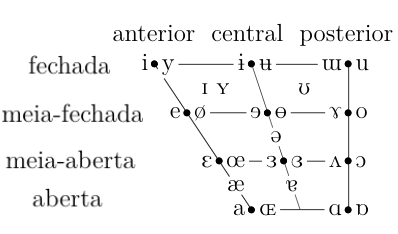
\includegraphics[width=0.45\linewidth]{img/vowels.png}
    \caption{Vogais IPA}
    \label{fig:vowels_ipa}
\end{figure}

A ideia do AFI é mapear e caracterizar todos os sons das línguas humanas. Desse modo, cada língua aproveita apenas um subconjunto do AFI. Os fones presentes no Português-Brasileiro estão circulados. Levando em conta apenas o subconjunto dos fones do PB, e também tendo em mente que os símbolos do alfabeto fonético precisam ser transformados em código ASCII para serem interpretados, faz sentido construir uma nova tabela adaptada para o problema em questão. O resultado desta adaptação pode ser visto nas Tabelas \ref{tab:new_rep} e \ref{tab:new_vocals}. Nessas novas tabelas, além da exclusão de alguns pontos e modos de articulação (motivada pela própria natureza do PB), apresenta-se também uma chave de transcrição alternativa que engloba apenas caracteres pertencentes ao código ASCII. Com relação à tabela das vogais (\ref{tab:new_vocals}), a dimensão de arredondamento foi dispensada pois não havia mais a necessidade dessa marcação.

\begin{center}
\scalebox{0.9}{
    \begin{tabular}{|l|cc|cc|cc|cc|cc|}
        \hline & 
            \multicolumn{2}{|c|}{\footnotesize{Bilabial}} &					% Bilabial
            \multicolumn{2}{|c|}{\footnotesize{Lab. dent.}} & 			% Labiodental
            \multicolumn{2}{|c|}{\footnotesize{Alveolar}} & 				% Alveolar
            \multicolumn{2}{|c|}{\footnotesize{P-alveo.}} & 		% Post-alveolar

            \multicolumn{2}{|c|}{\footnotesize{Velar}} & 					% Velar  \\				

        \hline Plosive &  							% Plosive
            p & b &	% Bilabial
            &&	% Labiodental
            t & d	% Alveolar
            & &% Post-alveolar
            & k & g 										         \\								

        \hline Nasal & 							% Nasal
            & m 	% Bilabial
            &  &  & % Labiodental
            & n 	% Alveolar
            & & % Post-alveolar
            & & N \\	% Velar
                     	

        \hline Tap/Flap &  						% Tap /Flap
            &													% Bilabial
            & &														% Labiodental
           && r &					% Alveolar
            &&                 % Post-alveolar

            \BlankCell        & &        	% Vela

        \hline Fricative & 						% Fricative
            &  &									% Bilabial
            f & v &													% Labiodental
            s & z &													% Alveolar
            x & j &									% Post-alveolar
            h  & \\										

        \hline Lat. appr. & 					% Lat. Approx
            \BlankCell        & \BlankCell        &		% Bilabial
            \BlankCell        & \BlankCell        &		% Labiodental

           & l &							% Alveolar
                                                      &&                  % Post-alveolar
  
             & L  	
             &% Velar
         
        \hline
    \end{tabular}
}%scalebox
\captionof{table}{Consoantes na nova representação}\label{tab:new_rep}
\end{center}

\begin{center}
\begin{table}[H]
\begin{center}
    \begin{tabular}{lll}
        \hline
         & Anterior & Posterior \\
         \hline
        Fechada & i & u \\
        \hline
        Meia-fechada & e & o \\
        \hline
        Meia-aberta & E & O \\
        \hline
        Aberta & a &  \\
        \hline
        Nasais & A (ã) &\\ & 3 ($\tilde{e}$) &\\ 
        \hline
    \end{tabular}
\end{center}
\caption{Vogais na nova representação}
\label{tab:new_vocals}
\end{table}
\end{center}


 A Tabela \ref{tab:chave} exibe a chave de transcrição proposta utilizando as tabelas  fonéticas criadas e a Tabela \ref{tab:transc} exibe alguns exemplos de transcrições possíveis.  

\begin{table}[H]
\begin{center}
\begin{tabular}{lc}
\textbf{AFI} & \multicolumn{1}{l}{\textbf{Transcrição Proposta}} \\ \hline

\textbf{{[}p{]}} - \textbf{p}arar & p \\
\textbf{{[}b{]}} - \textbf{b}otar & b \\
\textbf{{[}t{]}} - \textbf{t}ocar & t \\
\textbf{{[}d{]}} - \textbf{d}ançar & d \\
\textbf{{[}k{]}} - \textbf{c}asar & k \\
\textbf{{[}g{]}} - \textbf{g}ostar & g \\
\textbf{{[}f{]}} - \textbf{f}ugir & f \\
\textbf{{[}v{]}} - \textbf{v}oltar & v \\
\textbf{{[}s{]}} - \textbf{s}oltar & s \\
\textbf{{[}z{]}} - pre\textbf{s}enciar & z \\
\textbf{{[}\ipa{S}{]}} - \textbf{ch}amar & x \\
\textbf{{[}\ipa{Z}{]}} - \textbf{j}antar & j \\
\textbf{{[}t\ipa{S}{]}} - sen\textbf{t}ir & t \\
\textbf{{[}d\ipa{Z}{]}} - \textbf{d}izer & d \\
\textbf{{[}h{]}} - e\textbf{rr}ar & h \\
\textbf{{[}\ipa{\:r}{]}} - enca\textbf{r}ar & r \\
\textbf{{[}l{]}} - pu\textbf{l}ar & l \\
\textbf{{[}\textipa{L}{]}} - espa\textbf{lh}ar & L \\
\textbf{{[}m{]}} - \textbf{m}orar & m \\
\textbf{{[}n{]} }- \textbf{n}adar & n \\
\textbf{{[}\ipa{N}{]}} - so\textbf{nh}ar & N\\
\textbf{{[}a{]}} - p\textbf{a}rar & a \\
\textbf{{[}e{]}} - l\textbf{e}r & e \\
\textbf{{[}\textepsilon{]}} - esp\textbf{e}ro & E \\
\textbf{{[}i{]}} - r\textbf{i}r & i \\
\textbf{{[}o{]}} - pr\textbf{o}por & o \\
\textbf{{[}\textopeno{]} }- col\textbf{o}co & O \\
\textbf{{[}u{]}} - c\textbf{u}rtir & u \\
\textbf{{[}\~e{]}} - \textbf{e}ntreter & 3 \\
\textbf{{[}ã{]}} - pl\textbf{a}ntar & A \\
\textbf{{[}\~o{]}} - comp\textbf{o}nho & o \\
\textbf{{[}\textupsilon{]}} - cas\textbf{o} & u \\
\textbf{{[}j{]}} - sa\textbf{i}o & i \\
\textbf{{[}w{]}} - vo\textbf{l}to & u
\end{tabular}
\end{center}
\caption{Chave de Transcrição Proposta}
\label{tab:chave}
\end{table}

\begin{table}[H]
\begin{center}
\begin{tabular}{cc}
\hline
\textbf{Verbo} & \textbf{Transcrição} \\ \hline
ressentir & hes3ntir \\
paro & paru \\
possuo & posuu \\
olha & oLa \\
sacudir & sakudir \\
voltar & voutar \\ \hline
\end{tabular}
\end{center}
\caption{Exemplos de Transcrições}
\label{tab:transc}
\end{table}



\section{Corpus}
\label{sec:corpus}
O corpus utilizado para o treinamento dessa rede foi construído a partir da listagem de verbos contida no enderenço \texturl{www.conjugação.com.br}.

Primeiramente, foi realizada uma etapa de extração dos verbos e suas respectivas formas flexionadas para um arquivo \textit{.csv} via técnica de \textit{webscraping}, uma técnica que extrai informações contidas nas páginas da web (\cite{mitchell:2015}). Em seguida, os verbos irregulares foram selecionados manualmente para diferentes famílias de verbos, ou seja, grupos que continham o mesmo padrão de flexão. Alguns dos verbos irregulares listados na fonte de referência não eram irregulares no processo de flexão de interesse, e portanto foram realocados para o grupo de verbos regulares (vide exemplo do verbo \textit{correr} na Seção \ref{sec:escopo}). Na sequência, os verbos  coletados na forma infinitiva tiveram o fone /\textit{r}/ extraído para que no \textit{input} do modelo entrasse apenas o radical + vogal temática dos verbos.

 Um experimento foi realizado na tentativa de utilizar o transcritor fonético automático disponibilizado por \cite{guide:2016} para tornar o processo de transcrição mais rápido. Entretanto, o transcritor falhou na tentativa de transcrever verbos cujas escritas coincidem com substantivos, como por exemplo “apoio”, “peso”, “toco”, “posto”, “jogo”, entre outros. Desse modo, os verbos coletados foram transcritos manualmente utilizando a chave de transcrição apresentada na Tabela \ref{tab:chave}. No total, foram obtidos 423 verbos, 83 a menos que no experimento realizado por (\cite{rumelhart:1986}).

Dos 423 verbos extraídos, 20 foram considerados verbos sem possível agrupamento (verbos como “ir”, “trazer” e “saber”), totalizando uma base de 214 verbos regulares e 209 irregulares (50.6\% e 49.4\% respectivamente). A título de comparação, o estudo de \cite{rumelhart:1986} era composto por apenas 20\% de verbos irregulares.

A Tabela \ref{tab:classes} associa exemplos das classes obtidas à sua respectiva contagem e proporção no corpus.

\begin{table}[H]
\begin{center}
\begin{tabular}{|l|c|c|c|}
\toprule
 & Exemplos & Contagem & Proporção\\
\midrule
1  & ansia, anseio & 9 & 2.13\%\\
2  & bota, boto & 30 & 7.09\%\\
3  & cobri, cubro & 7 & 1.65\%\\
4  & dize, digo & 7 & 1.65\%\\
5 & faze, faço & 15 & 3.55\%\\
6  & cre, creio & 5 & 1.18\%\\
7  & senti, sinto & 8 & 1.89\% \\
8  & pedi, peço & 7 & 1.65\%\\
9  & pô, ponho & 27 & 6.38\%\\
10  & segui, sigo & 27 & 6.38\%\\
11  & te, tenho & 10 & 2.36\%\\
12  & testa, testo & 20 & 4.73\%\\
13  & ve, vejo & 6 & 1.42\%\\
14  & vi, venho & 10 & 2.60\%\\
15 & sabe, sei & 20 & 4.73\%\\
16  & fala, falo & 214 & 50.59\%\\
\bottomrule
\end{tabular}
\end{center}
\captionof{table}{Organização do corpus}
\label{tab:classes}
\end{table}

Apesar do volume de verbos irregulares ser consideravelmente maior do que o volume utilizado no estudo de \cite{rumelhart:1986}, pode-se dizer que algumas das famílias coletadas apresentam certa improdutividade, no sentido de que muitos verbos são reaproveitamentos de outros através do uso de prefixos. Por exemplo, a família do verbo “fazer” é composta apenas de verbos derivados do mesmo: “desfazer”, “refazer”, etc. Isto pode ser observado em outras classes, como a do verbo “cobrir”, “pedir”, “dizer”, “ver”, entre outras. As classes com maior variabilidade são as do verbo “botar” com por exemplo “tocar”, “gostar”, “colocar”; “testar” com “pegar”, “secar”, “testar”; e “seguir” com “digerir”, “regredir”, “divertir”.   

\subsection{Types x Tokens}
Outra questão importante a respeito do corpus utilizado, refere-se à frequência em que os verbos serão inseridos no modelo. Para isso, introduzimos os conceitos de \textit{word type} e \textit{word token} (\cite{Manning:1999}). Discutir sobre a frequência em que os verbos são inseridos é relevante, pois o treinamento das Redes Neurais se dá por meio de \textit{ciclos}. Como vimos no Cap. \ref{ch:01}, \cite{rumelhart:1986} conseguiram fabricar o comportamento da \textit{Curva de Desenvolvimento em U} ao manipular a frequência de inserção dos dados, privilegiando verbos irregulares. 

O termo \textit{type}, importado da área de \textit{Processamento de Linguagem Natural}, refere-se ao número de palavras \textbf{únicas} presentes em um Corpus. A frase “Essa frase é uma frase de exemplo.”, portanto, possui 6 \textit{types}. O termo \textit{token}, em contrapartida, refere-se ao número total de termos presentes, incluindo as repetições. Nesse caso, a mesma frase de exemplo possui 7 \textit{tokens}. 

Evidências na área de psicolinguística (\cite{Bybee:1995,janet:2018}) indicam que humanos aprendem a generalizar padrões fonológicos baseado na contagem de \textit{word types}, ignorando a frequência de uso das palavras. Com isso, nesta pesquisa cada verbo é visto como um \textit{word type}. Isso significa que a frequência de uso dos verbos não foi levada em consideração para a introdução dos mesmos no modelo. Ao invés disso, os verbos são tratados de forma igualitária e compartilham do mesmo número de inserções.\\


\subsection{Os Inputs do Modelo Encoder-Decoder}
\label{sec:inputs}

Após a construção do corpus, os verbos transcritos tiveram seus respectivos fones associados a um dicionário de traços fonéticos, os mesmos traços que originaram as Tabelas \ref{tab:new_rep} e \ref{tab:new_vocals}. A Tabela \ref{tab:pOsu} apresenta um exemplo desse processo para o verbo “posso” - “\textit{pOsu}”. 

\begin{table}[H]
\begin{center}
\begin{tabular}{lll}
Fone & Traços Fonéticos &  \\ \cline{1-2}
p & bilabial, oclusiva, surda &  \\
O & meio-aberta, posterior &  \\
s & fricativa, alveolar, surda &  \\
u & fechada, posterior & 
\end{tabular}
\end{center}
\caption{Traços Fonéticos para o Verbo “Posso“}
\label{tab:pOsu}
\end{table}

Na computação, um dicionário é uma estrutura de armazenamento de dados que associa uma chave a um valor. Essa estrutura possui um conjunto mutuamente exclusivo de chaves, cada uma associada a um valor. Desse modo, ao consultar um dicionário com um valor chave, a estrutura retorna como resposta o valor associado.

 No total são necessários 20 traços para representar um fone. São 18 para representar os traços das tabelas fonéticas construídas (\ref{tab:new_rep} e \ref{tab:new_rep}): Oclusivo, Nasal, Tepe, Fricativa, Aproximante Lateral, Bilabial, Labio-Dental, Alveolar, Pós-Alveolar, Velar, Glotal, Fechada, Meia-fechada, Meia-aberta, Aberta, Anterior, Posterior; e 2 para representar início e final do verbo ($<$beg$>$ e $<$end$>$).

Os fones são então caracterizados pela presença (1) e ausência (0) dos traços mencionados. Desse modo, o dicionário construído possui fones nos valores das chaves e uma lista de 0's e 1's para representar as presenças e ausências dos traços fonéticos. De acordo com as tabelas fonéticas desenvolvidas, cada fonema pode ser descrito por apenas três ou dois traços fonéticos, de modo que cada vetor terá apenas três ou dois valores marcados como \textbf{1}'s. Os \textit{tokens} de início e final do verbo ($<$beg$>$ e $<$end$>$) são exceções, com apenas uma marcação de \textbf{1} no vetor. 

A Tabela \ref{tab:coding_example} mostra como exemplo uma comparação entre dois fones similares (\textbf{p} e \textbf{b}) que distinguem-se apenas pelo traço fonético sonoro. O resultado é uma representação vetorial que também carrega essa noção de proximidade entre os fones. O começo do verbo é representado por um vetor que marca 0 em todos os traços fonéticos e 1 no \textit{token} de começo (o traço de fim pode ser compreendido de maneira análoga). 

\begin{table}[H]
\begin{center}
\begin{tabular}{lll}
\textbf{ Traço} & \textbf{p} &\textbf{ b} \\
 \toprule
oclusiva & 1 & 1 \\
nasal & 0 & 0 \\
tepe & 0 & 0 \\
fricativa & 0 & 0 \\
l-aprox & 0 & 0 \\
bilabial & 1 & 1 \\
labiodental & 0 & 0 \\
alveolar & 0 & 0 \\
p-alveolar & 0 & 0 \\
velar & 0 & 0 \\
glotal & 0 & 0 \\
sonora & 0 & 1 \\
fechada & 0 & 0 \\
m-fechada & 0 & 0 \\
m-aberta & 0 & 0 \\
aberta & 0 & 0 \\
anterior & 0 & 0 \\
posterior & 0 & 0 \\
<beg> & 0 & 0 \\
<end> & 0 & 0
\end{tabular}
\end{center}
\caption{Exemplo de Codificação de fones}
\label{tab:coding_example}
\end{table}

Por fim, juntando todos os passos expostos, o processo completo de transformação dos inputs pode ser resumido a:

\begin{enumerate}
    \item Adição dos \textit{tokens} de início e final dos verbos.
    \item Divisão dos verbos em fones, seguindo chave de transcrição proposta.
    \item Transformação dos fones em \textit{arrays} de 0's e 1's, seguindo o dicionário de fones desenvolvido.
\end{enumerate}







